% ===================================================================
%  Week 4 — Noise & Image Restoration
% ===================================================================
\documentclass[10pt,aspectratio=169]{beamer}
% ===================================================================
%  Shared Beamer preamble for "Practical Image Processing"
%  English slides. Compile with pdfLaTeX.
% ===================================================================

\usetheme{metropolis}
\usepackage[T1]{fontenc}
\usepackage[utf8]{inputenc}
\usepackage{lmodern}
\usepackage{listings}
\usepackage{tcolorbox}
\usepackage{fontawesome5}
\usepackage{booktabs}
\usepackage{amsmath,amssymb}
\usepackage{tikz}
\usepackage{pgfplots}
\pgfplotsset{compat=1.17}
\usetikzlibrary{arrows.meta,positioning,shapes.geometric,fit,backgrounds,matrix}
\tcbuselibrary{skins,breakable}

% ---- Palette --------------------------------------------------------
\definecolor{coursePrimary}{HTML}{1B4965}   % deep blue
\definecolor{courseAccent}{HTML}{E76F51}    % coral
\definecolor{courseGood}{HTML}{2A9D8F}      % teal
\definecolor{courseBad}{HTML}{C0392B}       % red
\definecolor{courseInfo}{HTML}{2980B9}      % blue
\definecolor{codeBg}{HTML}{F5F6FA}
\definecolor{codeKw}{HTML}{8E44AD}
\definecolor{codeStr}{HTML}{2A9D8F}
\definecolor{codeCom}{HTML}{7F8C8D}

\setbeamercolor{frametitle}{bg=coursePrimary}
\setbeamercolor{progress bar}{fg=courseAccent}
\setbeamercolor{alerted text}{fg=courseAccent}
\metroset{block=fill,sectionpage=progressbar,numbering=fraction}

% ---- Code listings (Python is built into listings) -----------------
\lstdefinestyle{course}{
  backgroundcolor=\color{codeBg},
  basicstyle=\ttfamily\scriptsize,
  keywordstyle=\color{codeKw}\bfseries,
  stringstyle=\color{codeStr},
  commentstyle=\color{codeCom}\itshape,
  numberstyle=\tiny\color{codeCom},
  numbers=left, numbersep=6pt,
  showstringspaces=false, breaklines=true, breakatwhitespace=true,
  tabsize=4, columns=fullflexible,
  frame=single, framesep=4pt, rulecolor=\color{gray!30},
  keepspaces=true, upquote=true, language=Python,
}
\lstset{style=course}
\lstdefinelanguage{bash}{
  keywords={cd,pip,python,venv,source,import}, sensitive=true,
  morecomment=[l]{\#}, morestring=[b]', morestring=[b]",
}

% ---- Reusable callout boxes ----------------------------------------
\newtcolorbox{goodbox}[1][Good practice]{colback=courseGood!8,colframe=courseGood,
  fonttitle=\bfseries,title={\faCheck~#1},boxrule=0.6pt,left=4pt,right=4pt,top=3pt,bottom=3pt}
\newtcolorbox{badbox}[1][Pitfall]{colback=courseBad!8,colframe=courseBad,
  fonttitle=\bfseries,title={\faTimes~#1},boxrule=0.6pt,left=4pt,right=4pt,top=3pt,bottom=3pt}
\newtcolorbox{infobox}[1][Note]{colback=courseInfo!8,colframe=courseInfo,
  fonttitle=\bfseries,title={\faInfoCircle~#1},boxrule=0.6pt,left=4pt,right=4pt,top=3pt,bottom=3pt}
\newtcolorbox{mathbox}[1][Math]{colback=coursePrimary!6,colframe=coursePrimary,
  fonttitle=\bfseries,title={\faCalculator~#1},boxrule=0.6pt,left=4pt,right=4pt,top=3pt,bottom=3pt}

\newcommand{\keyidea}[1]{\begin{alertblock}{Key idea}#1\end{alertblock}}
\newcommand{\term}[1]{\textbf{\color{coursePrimary}#1}}
\newcommand{\code}[1]{\lstinline[basicstyle=\ttfamily\small]|#1|}

% ---- A helper to draw a small pixel grid, cells shaded by value ----
% \pixelgrid{ {10,20,120,200,240}, {30,60,130,180,230}, ... }
\newcommand{\pixelgrid}[1]{%
  \begin{tikzpicture}[font=\scriptsize,scale=0.6]
    \foreach \row [count=\ry] in {#1} {
      \foreach \val [count=\cx] in \row {
        \draw[gray,fill=coursePrimary!8] (\cx,-\ry) rectangle ++(1,-1);
        \node at (\cx+0.5,-\ry-0.5) {\val};
      }
    }
  \end{tikzpicture}}


\title{Noise \& Restoration}
\subtitle{Week 4 — Modelling and removing noise}
\author{Practical Image Processing}
\date{Lecture 4 \textbullet\ 60--70 min}

\begin{document}

\maketitle

\begin{frame}{Recap \& today}
  \begin{columns}[T]
    \begin{column}{0.58\textwidth}
      \begin{itemize}
        \item Wk3: filters combine a pixel with its neighbours (convolution).
        \item \alert{Today:} \term{noise} — where it comes from, how to \term{model} it, and how
              to \term{remove} it without destroying the detail you need.
      \end{itemize}
    \end{column}
    \begin{column}{0.42\textwidth}
      \begin{alertblock}{Why it matters}
        Real meter photos are noisy (low light, high ISO). Denoising is what makes the digits
        thresholdable and readable.
      \end{alertblock}
    \end{column}
  \end{columns}
\end{frame}

\begin{frame}{Roadmap}\tableofcontents\end{frame}

% ==================================================================
\section{Noise models}
% ==================================================================

\begin{frame}{Two noises you must recognize}
  \begin{columns}[T]
    \begin{column}{0.33\textwidth}\begin{center}
      
\includegraphics[width=\linewidth]{../assets/clean.png}\\{\scriptsize clean}
    \end{center}\end{column}
    \begin{column}{0.33\textwidth}\begin{center}
      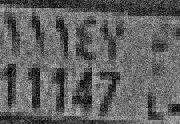
\includegraphics[width=\linewidth]{../assets/gaussian_noise.png}\\{\scriptsize Gaussian}
    \end{center}\end{column}
    \begin{column}{0.33\textwidth}\begin{center}
      
\includegraphics[width=\linewidth]{../assets/sp_noise.png}\\{\scriptsize salt-and-pepper}
    \end{center}\end{column}
  \end{columns}
  \vspace{3pt}
  \keyidea{The noise \emph{type} decides the \emph{cure}. Gaussian $\rightarrow$ averaging; impulse $\rightarrow$ median. Diagnose first.}
\end{frame}

\begin{frame}{Where noise comes from (physics, Week 1)}
  \begin{itemize}
    \item \term{Gaussian noise}: small random fluctuations added to every pixel (sensor/read noise).
    \item \term{Salt-and-pepper} (impulse): random pixels stuck at 0 or 255 (dead pixels, transmission).
    \item \term{Poisson} (shot) noise: from photon counting; stronger in dark areas / low light.
  \end{itemize}
  \begin{mathbox}
    Gaussian model: $g = f + n$, with $n\sim\mathcal{N}(0,\sigma^2)$ — additive and zero-mean.
  \end{mathbox}
\end{frame}

\begin{frame}{Diagnosing noise}
  \begin{itemize}
    \item Look at a \term{flat} region: Gaussian = a fuzzy spread; salt-pepper = isolated black/white specks.
    \item The histogram of a flat patch: Gaussian widens the peak; impulse adds spikes at 0 and 255.
    \item Match the filter to what you see — using the wrong one wastes detail or fails to clean.
  \end{itemize}
  \begin{badbox}
    Averaging (Gaussian blur) barely touches salt-and-pepper — it just spreads each speck into a gray smudge.
  \end{badbox}
\end{frame}

% ==================================================================
\section{Restoration}
% ==================================================================

\begin{frame}{Removing Gaussian noise}
  \begin{columns}[T]
    \begin{column}{0.25\textwidth}\begin{center}
      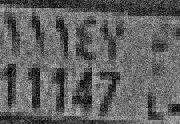
\includegraphics[width=\linewidth]{../assets/gaussian_noise.png}\\{\scriptsize noisy}
    \end{center}\end{column}
    \begin{column}{0.25\textwidth}\begin{center}
      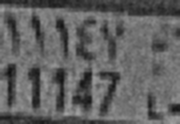
\includegraphics[width=\linewidth]{../assets/gauss_denoise_gauss.png}\\{\scriptsize Gaussian blur}
    \end{center}\end{column}
    \begin{column}{0.25\textwidth}\begin{center}
      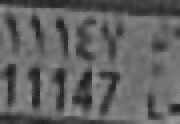
\includegraphics[width=\linewidth]{../assets/gauss_denoise_bilateral.png}\\{\scriptsize bilateral}
    \end{center}\end{column}
    \begin{column}{0.25\textwidth}\begin{center}
      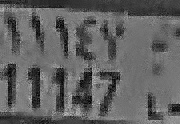
\includegraphics[width=\linewidth]{../assets/gauss_denoise_nlm.png}\\{\scriptsize non-local means}
    \end{center}\end{column}
  \end{columns}
  \vspace{3pt}
  Gaussian blur smooths but blurs edges; bilateral keeps edges; NLM is best but slowest.
\end{frame}

\begin{frame}{Removing salt-and-pepper — median wins}
  \begin{columns}[T]
    \begin{column}{0.33\textwidth}\begin{center}
      
\includegraphics[width=\linewidth]{../assets/sp_noise.png}\\{\scriptsize noisy}
    \end{center}\end{column}
    \begin{column}{0.33\textwidth}\begin{center}
      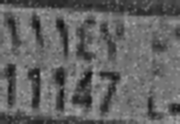
\includegraphics[width=\linewidth]{../assets/sp_denoise_gauss.png}\\{\scriptsize Gaussian (bad)}
    \end{center}\end{column}
    \begin{column}{0.33\textwidth}\begin{center}
      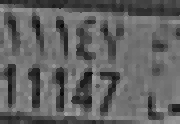
\includegraphics[width=\linewidth]{../assets/sp_denoise_median.png}\\{\scriptsize median (great)}
    \end{center}\end{column}
  \end{columns}
  \vspace{3pt}
  \keyidea{The median ignores outliers: a speck of 255 among 100s doesn't move the median.
  This is why median crushes impulse noise while keeping edges.}
\end{frame}

\begin{frame}{Why median beats averaging for impulse noise}
  \begin{itemize}
    \item Mean of $\{100,100,100,255\}$ = 164 — the outlier drags it up.
    \item Median of the same = 100 — the outlier is ignored entirely.
    \item Averaging \emph{spreads} an impulse; median \emph{deletes} it. Match filter to noise.
  \end{itemize}
  \begin{mathbox}
    Median is robust to outliers; the mean is not. That single fact explains the whole result.
  \end{mathbox}
\end{frame}

\begin{frame}{Bilateral \& non-local means}
  \begin{itemize}
    \item \term{Bilateral}: average only neighbours of \emph{similar intensity} $\rightarrow$ smooth flats, keep edges.
    \item \term{Non-local means (NLM)}: average pixels with a similar \emph{neighbourhood pattern}, anywhere in the image.
    \item NLM gives the best quality on Gaussian noise, at a real speed cost.
  \end{itemize}
  \begin{goodbox}
    For DocScan: bilateral or NLM before thresholding keeps digit edges crisp while killing sensor grain.
  \end{goodbox}
\end{frame}

\begin{frame}{A quick reference of noise $\rightarrow$ filter}
  \begin{center}
  \begin{tabular}{@{}lll@{}}
    \toprule
    \textbf{Noise} & \textbf{Looks like} & \textbf{Best filter} \\
    \midrule
    Gaussian & fuzzy grain everywhere & Gaussian / NLM \\
    Salt-and-pepper & isolated black/white dots & median \\
    Poisson (shot) & grain, worse in dark & NLM / variance-stabilize \\
    Periodic & repeating wave/pattern & frequency-domain (Week 6) \\
    \bottomrule
  \end{tabular}
  \end{center}
  \keyidea{Periodic noise is invisible to spatial filters — you remove it in the frequency domain (Week 6).}
\end{frame}

\begin{frame}[fragile]{Denoising in code}
\begin{lstlisting}[language=Python]
gauss     = cv2.GaussianBlur(noisy, (5,5), 0)
median    = cv2.medianBlur(noisy, 3)             # salt-and-pepper
bilateral = cv2.bilateralFilter(noisy, 9, 60, 60)  # edge-preserving
nlm       = cv2.fastNlMeansDenoising(noisy, None, 15, 7, 21)  # best, slow
\end{lstlisting}
  \begin{infobox}
    Try median first for specks; bilateral/NLM when you must keep edges. Measure, don't guess.
  \end{infobox}
\end{frame}

% ==================================================================
\section{In-class exercise}
% ==================================================================

\begin{frame}{\faPen~In-class exercise (10 min)}
  \begin{infobox}[Pick the filter]
  \end{infobox}
  For each situation, which filter and why?
  \begin{enumerate}
    \item A scanned meter with random black/white dots.
    \item A low-light phone photo with fine grain everywhere.
    \item A document where you must keep the text edges razor-sharp while removing grain.
    \item How would you \emph{measure} whether your denoising actually helped?
  \end{enumerate}
\end{frame}

\begin{frame}{\faPen~Debrief}
  \begin{itemize}
    \item (1) Salt-and-pepper $\rightarrow$ \term{median}. (2) Gaussian grain $\rightarrow$ Gaussian/NLM.
    \item (3) Edge-preserving $\rightarrow$ \term{bilateral} (or NLM). (4) Measure with \term{PSNR}/SSIM vs a clean reference, or by downstream OCR accuracy.
    \item Golden rule: the \term{cheapest} filter that removes the noise \emph{your} pipeline cares about.
  \end{itemize}
  \keyidea{``Denoise'' isn't one button — it's choosing the model that matches the noise.}
\end{frame}

% ==================================================================
\section{Deep dive}
% ==================================================================

\begin{frame}{Measuring restoration: PSNR \& SSIM}
  \begin{itemize}
    \item \term{PSNR}: based on mean-squared error vs a clean reference; higher = closer (in dB).
    \item \term{SSIM}: perceptual — compares structure, not just pixel errors; better matches human judgment.
    \item If you have a clean reference (or a synthetic-noise experiment), \emph{measure}, don't eyeball.
  \end{itemize}
  \begin{mathbox}
    $\mathrm{PSNR}=10\log_{10}\dfrac{255^2}{\mathrm{MSE}}$
  \end{mathbox}
\end{frame}

\begin{frame}{The denoising dilemma}
  \begin{itemize}
    \item Every denoiser trades \term{noise removal} against \term{detail preservation}.
    \item Remove too little $\rightarrow$ noise breaks the next stage; too much $\rightarrow$ you erase the digits.
    \item There is no free lunch: choose the operating point for \emph{your} goal (readable digits).
  \end{itemize}
  \keyidea{Denoise for the downstream task, measured on hard images — not for the prettiest flat wall.}
\end{frame}

\begin{frame}{Temporal denoising: average many frames}
  \begin{itemize}
    \item If you have several shots of the \emph{same} static scene, average them: noise cancels, signal stays.
    \item $N$ frames reduce Gaussian noise by $\sqrt{N}$ — the cheapest, highest-quality denoiser.
    \item For a meter you can photograph twice, this beats any single-image filter.
  \end{itemize}
  \begin{goodbox}
    When you control capture, averaging a burst is the best denoising you can do — no detail lost.
  \end{goodbox}
\end{frame}

\begin{frame}{Restoration vs enhancement}
  \begin{itemize}
    \item \term{Enhancement} (Wk2) makes an image \emph{look} better (subjective).
    \item \term{Restoration} tries to \emph{recover} the original by modelling the degradation (objective).
    \item Deblurring is restoration too: if you know the blur (the \term{PSF}), you can partly invert it.
  \end{itemize}
\end{frame}

\begin{frame}{Deblurring \& the PSF (brief)}
  \begin{itemize}
    \item Blur = convolution with a \term{point-spread function} (PSF). Deblur = deconvolution.
    \item Naive inversion amplifies noise catastrophically; real methods (Wiener, Richardson-Lucy) regularize.
    \item Motion/defocus blur on a meter photo is often better \emph{avoided} (steady shot) than fixed.
  \end{itemize}
  \begin{badbox}
    Perfect deblurring is impossible when information is truly lost. Prevention beats restoration.
  \end{badbox}
\end{frame}

\begin{frame}{Where denoising sits in the pipeline}
  \begin{center}
  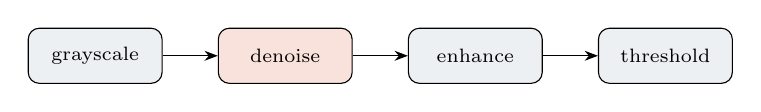
\begin{tikzpicture}[font=\scriptsize,>=Stealth,node distance=3mm and 7mm,
    b/.style={draw,rounded corners,fill=coursePrimary!8,minimum height=7mm,minimum width=17mm,align=center}]
    \node[b] (load){grayscale};
    \node[b,right=of load,fill=courseAccent!20] (den){denoise};
    \node[b,right=of den] (enh){enhance};
    \node[b,right=of enh] (thr){threshold};
    \draw[->](load)--(den);\draw[->](den)--(enh);\draw[->](enh)--(thr);
  \end{tikzpicture}
  \end{center}
  \begin{itemize}
    \item Denoise \emph{early} — before enhancement (which would amplify the noise) and before thresholding (which noise would corrupt).
    \item But not \emph{too} aggressively: over-denoising erases the digits you need.
  \end{itemize}
\end{frame}

\begin{frame}{Adaptive \& order-statistic filters}
  \begin{itemize}
    \item \term{Adaptive median}: grows its window only where noise is detected — cleans heavy impulse noise with less blur.
    \item \term{Min/Max} filters: remove pepper (min) or salt (max) specifically.
    \item These are the ``order-statistic'' family — like median, they pick a ranked value, not an average.
  \end{itemize}
  \begin{goodbox}
    For very noisy meter scans, an adaptive median can save digits a plain median would smear.
  \end{goodbox}
\end{frame}

\begin{frame}{Deep learning denoisers (preview)}
  \begin{itemize}
    \item Modern denoisers are CNNs trained on (noisy, clean) pairs — they beat classical methods.
    \item But they need data, compute, and can \emph{hallucinate} detail that isn't there.
    \item For DocScan, classical (median/bilateral/NLM) is usually enough and fully interpretable.
  \end{itemize}
\end{frame}

% ==================================================================
\section{Wrap-up}
% ==================================================================

\begin{frame}{What you should now be able to do}
  \begin{itemize}
    \item Recognize Gaussian vs impulse noise and name their physical origins.
    \item Choose the matching filter (median / Gaussian / bilateral / NLM).
    \item Measure restoration with PSNR/SSIM instead of eyeballing.
    \item Reason about the noise-vs-detail trade-off for your pipeline.
  \end{itemize}
\end{frame}

\begin{frame}{This week's deliverable}
  \begin{alertblock}{Due before Week 5 (see \code{project/})}
    \begin{enumerate}
      \item Add Gaussian and salt-pepper noise to a clean meter image (known noise = ground truth).
      \item Denoise each with 3 filters; compute PSNR vs the clean original; tabulate.
      \item Show a case where the ``wrong'' filter fails (Gaussian on salt-pepper).
      \item DocScan: denoise a real noisy meter photo so its Otsu/adaptive binary is clean.
    \end{enumerate}
  \end{alertblock}
\end{frame}

\begin{frame}[standout]
  Match the filter to the noise.\\[4pt]
  \normalsize Median for specks, averaging for grain, bilateral to keep edges.
\end{frame}

\end{document}
